\chapter{\sffamily Probabilistic online learning software}

{\bfseries\sffamily Concept.} To outline the software design characteristics of a probabilistic online learning framework, built to interface directly with our generalised simulation engine. The probabilistic algorithms we introduced in the previous chapter will form the basic set of tools in this framework. As well as its own implementations of some learning algorithms, this software is also designed to enable interoperability with other machine learning APIs, e.g., Libtorch (via Gotch), and optimisation libraries, e.g., Gonum and eaopt. For the mathematically-inclined, this chapter will motivate online learning as an essential framework for our use case and how our probabilistic algorithms can work within this context. For the programmers, the software designed and described in this chapter lives in this public Git repository: \href{https://github.com/umbralcalc/learnadex}{https://github.com/umbralcalc/learnadex}.

\section{\sffamily Online learning with any algorithm}

In the previous chapter we motivated the use of some probabilistic learning methods, but we haven't yet discussed how we might implement them in practice. In particular, before discussing the software design aspects, we need to consider how we might structure learning by optimisation of Eq.~(\ref{eq:log-likelihood-reweighting}) for a sequence of observations in time. 

One of the issues that can arise when learning streams of data is `concept drift'. In our context, this would be when the optimal value for $z$ does not match the optimal value at some later point in time. In order to mitigate this, our learning algorithms should be able to track an up-to-date optimal value for $z$ as data is continually passed into them. Iteratively updating the optimal parameters as new data is ingested into the objective function is typically called `online learning'~\cite{hazan2016introduction,sutton2018reinforcement}, in contrast to `offline learning' which would correspond to learning an optimal $z$ only once with the entire dataset provided upfront.\footnote{This book will mostly be focussed on using online learning techniques due to the inherently sequential nature of stochastic processes.}

The reader may recall that this book is about building more realistic environments for machine learning systems; an important part of learning from environments in a robust manner is \emph{adaptability}.

\textcolor{red}{Got to here in rewrite...}

\section{\sffamily Software design}

Let's now take a step back from the specifics of the probabilistic reweighting algorithm to introduce our new sofware package for this part of the book: the `learnadex'. At its core, the learnadex algorithm adapts the stochadex iteration engine to iterate through streams of data in order to accumulate a global objective function value with respect to that data. The user may then choose which optimisation algorithm (or write their own) to use in order to leverage this objective for learning a better representation of the data. 

As we discussed at the end of the last section, the algorithms in the learnadex are all applied in an `online' fashion --- refitting for the optimal hyperparameters $z$ as new data is streamed into them. A challenging aspect of online learning is in managing the computational expense of recomputing the optimal value for $z$ after each new datapoint is sent. To help with this; the user may configure the algorithm recompute the optimum value after larger batches of data have been ingested. The last value of optimum $z$ will also frequently be close to the next optimum in the sequence, so using the former as the initial input into the optimisation routine for the latter is typically very valuable for aiding efficiency.

Reusing the \texttt{PartitionCoordinator} code of the stochadex to facilitate online learning makes neat use of software which has already been designed and tested in earlier chapters of this book. However, in order to fully achieve this, a few minor extensions to the typing structures and code abstractions are necessary; as we show in Fig.~\ref{fig:learnadex-data-types-design}. To start with, we separate out `learning' from the kind of optimiser in the overall config so as to enable multiple optimisation algorithms to be used for the same learning problem. The hyperparameters that define that optimisation problem domain can be determined by the user with an extension to the \texttt{OtherParams} object so that it includes some optional Boolean masks over the parameters, i.e., \texttt{OtherParams.FloatParamMask} and \texttt{OtherParams.IntParamMask}. These masks are used to extract the parameters of interest, which can then be flattened and formatted to fit into any generic optimisation algorithm.

\begin{figure}[h]
\centering
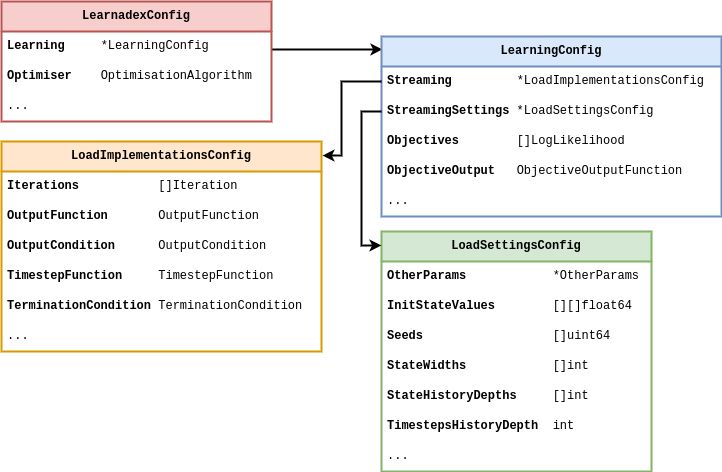
\includegraphics[width=12cm]{images/chapter-3-learnadex-data-types.drawio.png}
\caption{A relational summary of the core data types in the learnadex.}
\label{fig:learnadex-data-types-design}
\end{figure}

On the learning side; in order to define a specific objective for each data iterator to compute while the data streams through it, we have abstracted a `log-likelihood' type. Similarly, each iterator also gets a data streamer configuration which defines where the data is streaming from --- e.g., from a file on disk, from a local database instance or maybe via a network socket --- and also some inherited abstractions from the stochadex which define the time stepping function and when the data stream ends. In Fig.~\ref{fig:learnadex-data-iterator} below, we provide a schematic of the method calls of (and within) each data iterator.

\textcolor{red}{\begin{itemize}
\item{introduce the $\beta$ past discounting factor in this section and explain what it's for}
\item{refactor the code so that it's always doing online learning under the hood --- this can either be rolling refits in blocks on a refitting schedule with any optimisation algorithm of choice or full online learning Adam optimisation $$z_*({\sf t}+1) = -\alpha [{\sf t}+1,\text{stats of gradient history like Adam}] \frac{\partial}{\partial z} \ln {\cal L}_{{\sf t}+1} + z_*({\sf t})$$}
\item{refactor the code and integrate the reweighting algorithm with Libtorch models for the conditional probabilities --- describe how this is supported}
\item{describe the method calls diagram in more detail --- in particular, point out how it can replace the \texttt{Iteration.Iterate} method which is called when the \texttt{StateIterator} is asked for another iteration from the \texttt{PartitionCoordinator} of the stochadex}
\item{then talk about the optimiser! starting with non-gradient-based: the two packages that are supported out of the box are gonum and eaopt (still need to do gago --- see here: github.com/maxhalford/eaopt) }
\item{also need to then support gradient-based algorithms (like vanilla SGD) by implementing Eq.~(\ref{eq:log-likelihood-reweighting-grad}) for the current basic implementations in the learnadex --- shouldn't be too difficult!}
\item{then talk about the output - talk about the possibilities for output and what the default setting to json logs is for}
\item{could also be written to, e.g., a locally-hosted database server and the best-suited would be a NoSQL document database, e.g., MongoDB~\cite{mongodb}, but building something bespoke and simpler is more aligned with the use-case here and with the principles of this book}
\item{describe the need for log exploration and visualisation and then introduce logsplorer - a REST API for querying the json logs (with basic filtering and selection capabilities but could be extended to more advanced options) and optionally also launches a visualisation React app written in Typescript}
\item{note how this could be scaled to cloud services easily and remotely queried through the logsplorer API and visualised} 
\end{itemize}}

\begin{figure}[h]
\centering
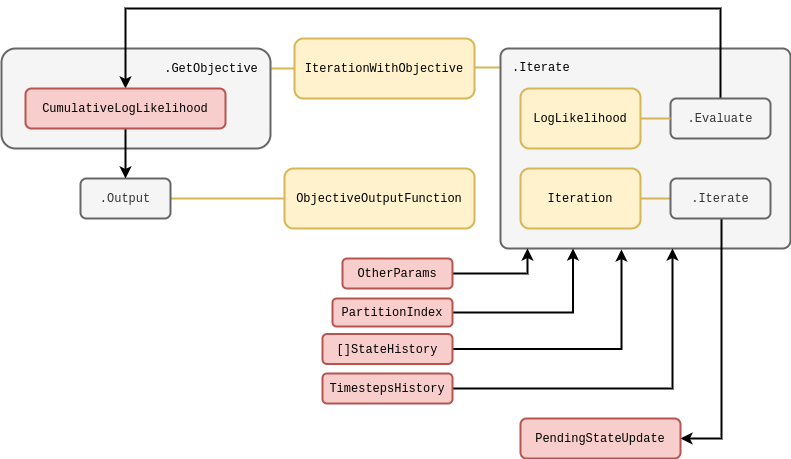
\includegraphics[width=14cm]{images/chapter-3-learnadex-data-iterator.drawio.png}
\caption{A schematic of an iteration with an objective function evaluation.}
\label{fig:learnadex-data-iterator}
\end{figure}

As with the software we wrote for the stochadex, the learnadex main binary executable leverages templating to enable full configurability of all the implementations and settings of Fig.~\ref{fig:learnadex-data-types-design} through passing configs at runtime. Users can alternatively use the learnadex as a library for import, if they desire more control over the code execution. 

\begin{figure}[h]
\centering
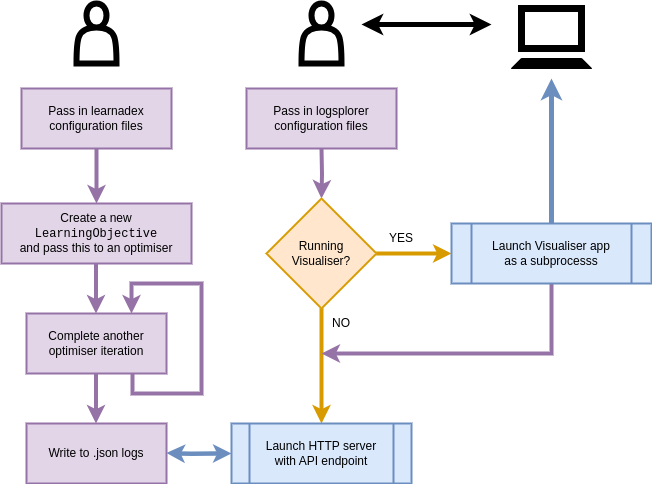
\includegraphics[width=13cm]{images/chapter-3-learnadex-main.drawio.png}
\caption{A diagram of the main learnadex and logsplorer executables.}
\label{fig:learnadex-main}
\end{figure}
    